\documentclass[%
% reprint,
superscriptaddress,
% groupedaddress,
% unsortedaddress,
% runinaddress,
% frontmatterverbose,
preprint,
preprintnumbers,
% nofootinbib,
% nobibnotes,
bibnotes,
amsmath,
amssymb,
aps,
showkeys,
% pra,
prb,
% rmp, prstab, prstper, floatfix,
]{revtex4-1}

\usepackage{braket}
\usepackage{graphicx}
\graphicspath{{images_inkscape/}}
\usepackage{dcolumn}                    % Align table columns on decimal point
\usepackage{bm}                         % bold mathb
\usepackage{hyperref}                   % add hypertext capabilities
\usepackage[mathlines]{lineno}          % Enable numbering of text and display math
% \linenumbers\relax                    % Commence numbering lines

% \usepackage[showframe,%Uncomment any one of the following lines to test
% scale=0.7, marginratio={1:1, 2:3}, ignoreall,% default settings
% text={7in,10in},centering,
% margin=1.5in,      total={6.5in,8.75in},      top=1.2in,      left=0.9in,      includefoot,
% height=10in,a5paper,hmargin={3cm,0.8in},
% ]{geometry}

%% Common Packages
\usepackage[usenames,dvipsnames,svgnames,table,rgb]{xcolor} % for colouring \color{red!20}
\usepackage{framed}         	% \begin{framed} for framed boxes
\usepackage{multirow}               % merge rows in tables

%%% COLOURS
\newcommand{\red}[1]{{\color{red}{#1}}}
\newcommand{\blue}[1]{\textcolor{blue}{#1}}
\newcommand{\green}[1]{\textcolor{green}{#1}}
\newcommand{\purple}[1]{\textcolor{purple}{#1}}
\newcommand{\grey}[1]{{\color{gray!60} #1}}
\newcommand{\ec}{ }                             % end colour command for emacs regexp
\definecolor{amber}{rgb}{1.0, 0.75, 0.0}
\newcommand{\gold}[1]{{\color{amber}{#1}}}

%%% Physics
% Bra and Ket
\newcommand{\iket}[1]{\ensuremath{\Ket{#1}}}
\newcommand{\ibra}[1]{\ensuremath{\Bra{#1}}}
\newcommand{\iketbra}[2]{\ket{#1}\bra{#2}}
\newcommand{\iup}{\ensuremath{\Ket{\uparrow}}}
\newcommand{\idown}{\ensuremath{\Ket{\downarrow}}}
\newcommand{\iupBra}{\ensuremath{\Bra{\uparrow}}}
\newcommand{\idownBra}{\ensuremath{\Bra{\downarrow}}}
\newcommand{\iupKetBra}{\ensuremath{\Ket{\uparrow}\Bra{\uparrow}}}
\newcommand{\idownKetBra}{\ensuremath{\Ket{\downarrow}\Bra{\downarrow}}}
% matrices
\newcommand{\iz}{\ensuremath{\begin{pmatrix}1&0\\0&-1\end{pmatrix}}}
\newcommand{\ix}{\ensuremath{\begin{pmatrix}0&1\\1&0\end{pmatrix}}}
\newcommand{\iy}{\ensuremath{\begin{pmatrix}0&-i\\i&0\end{pmatrix}}}
\newcommand{\idensity}{\ensuremath{\begin{pmatrix}{\rho_{00}} & {\rho_{01}}\\{\rho_{10}}&{\rho_{11}}\end{pmatrix}}}

% symbols
\newcommand{\isigma}{\ensuremath{\vec{\iaverage{\sigma}}}}
\newcommand{\isigmax}{\ensuremath{{\iaverage{\sigma_x}}}}
\newcommand{\isigmay}{\ensuremath{{\iaverage{\sigma_y}}}}
\newcommand{\isigmaz}{\ensuremath{{\iaverage{\sigma_z}}}}
\newcommand{\iadagger}{\ensuremath{a^{\dagger}}}
\newcommand{\isigmaplus}{\ensuremath{\iaverage{\sigma^{+}}}}
\newcommand{\isigmaminus}{\ensuremath{\iaverage{\sigma^{-}}}}
\newcommand{\isigmaplusminus}{\ensuremath{\iaverage{\sigma^{\pm}}}}


%%% Math simplicity
\newcommand{\iunit}[2]{\ensuremath{#1\,\text{#2}}}
\newcommand{\iunitMixed}[3]{\ensuremath{#1\,#2\text{#3}}}
\newcommand{\iabsSquared}[1]{\ensuremath{\left|#1\right|^2}}
\newcommand{\iabs}[1]{\ensuremath{\left|#1\right|}}
\newcommand{\icommutation}[2]{\ensuremath{\left[#1,                                #2\right]}}
\newcommand{\iaverage}[1]{\ensuremath{\left\langle #1 \right\rangle}}
\newcommand{\iderivative}[2]{%
  \ensuremath{%
    \frac{\partial#1}{\partial#2}}}
\newcommand{\ira}{\ensuremath{\,\rightarrow\,}}
\newcommand{\iRa}{\ensuremath{\qquad\Rightarrow\qquad}}
\newcommand{\ilra}{\ensuremath{\,\leftrightarrow\,}}
\newcommand{\iratext}[1]{\ensuremath{\,\xrightarrow{\text{#1}}\,}}

\begin{document}

\title{Supplementary Notes: The superconducting twin qubit}
% \thanks{A footnote to the article title}%

\author{I.  V.  Antonov}  \affiliation{Royal Holloway, University of London,  Egham, TW20 0EX,
  UK} \affiliation{National Physical Laboratory, Hampton Road Teddington, TW11 0LW, UK}

\author{R. S.  Shaikhaidarov} \affiliation{Royal Holloway,  University of London,  Egham, TW20
  0EX, UK}

\author{V.  N.  Antonov} \affiliation{Skolkovo Institute of Science and Technology, Nobel str.
  3, Moscow,  143026, Russia} \affiliation{Royal  Holloway, University of London,  Egham, TW20
  0EX,  UK} \affiliation{Moscow  Institute of  Physics and  Technology, 29  Institutskiy per.,
  141700 Dolgoprudny, Moscow Region, Russia}

\author{O.V.  Astafiev} \affiliation{Skolkovo Institute of  Science and Technology, Nobel str.
  3, Moscow,  143026, Russia} \affiliation{Royal  Holloway, University of London,  Egham, TW20
  0EX, UK} \affiliation{National Physical Laboratory, Hampton Road Teddington, TW11 0LW, UK}

\date{\today}% It is always \today, today,

\maketitle
% \date{\today}
% \author{I.  V.  Antonov}  \affiliation{Royal Holloway, University of London,  Egham, TW20 0EX,
%   UK} \affiliation{National Physical Laboratory, Hampton Road Teddington, TW11 0LW, UK}
% \begin{abstract}
% \end{abstract}

% \section{Decoherence results in loss of quantum information}
% \label{sec:decoh-results-loss}

% \noindent Quantum  processing involves manipulating  the state of  a qubit, $\Psi$,  changing the
% relative state population, $\ensuremath{|\alpha|} \le 1$, and phase, $\varphi$, between states \iket{0} and
% \iket{1}:
% \begin{equation}
%   \label{eq:4}
%   \Psi = \alpha\iket{0} + e^{i\varphi}(1-\alpha)\iket{1}.
% \end{equation}

% \noindent  When  written as  a  density  matrix, the  phase  information  is mapped  onto  the
% off-diagonal elements:
% \begin{equation}
%   \label{eq:5}
%   \rho = \iketbra{\Psi}{\Psi} = \begin{pmatrix}
%     \iabsSquared{\alpha}  & \alpha(1-\alpha)e^{-i\varphi}\\
%     \alpha(1-\alpha)e^{+i\varphi} & \iabsSquared{(1-\alpha)}.
%   \end{pmatrix}
% \end{equation}

% \noindent Decoherence,  by definition, causes  the off-diagonal elements  decay to 1/e  of the
% initial  value over  a time  $\tau_{\text{DECs}}$. Decoherence  causes the  loss of  computational
% information encoded in the phase $\varphi$.

\section{Capacitance matrix}
\label{sec:capacitance-matrix}

We are considering a capacitance network of the qubit, shown in Fig. (1). Each Josephson junction has capacitance $C_{ij}$, where $i$ and $j$ are island numbers (0, 1, 2, 3). The corresponding capacitance matrix is
  \begin{equation}
\bold{C} =  \begin{pmatrix}
      C_{01} + C_{12}& -C_{12} & 0\\
      -C_{12} & C_{12} + C_{02} + C_{23} + C_c & -C_{23}\\
      0 & -C_{23} & C_{03} + C_{23}
    \end{pmatrix}
    .
  \end{equation}
All Josephson junctions except the central one are identical and equal to $C$: $C_{01} = C_{12} = C_{03} = C_{23} = C$. The central junction is different, which together with small coupling capacitance $C_c$ can be represented as $C_{02} + C_c = \alpha' C$. Note that $C_c \ll C$ and $\alpha' \approx \alpha$.    
The capacitance matrix is simplified to 
\begin{framed}\noindent
  \begin{equation}
\bold{C} =  C \begin{pmatrix}
      2 & -1 & 0\\
      -1 & 2 + \alpha & -1\\
      0 & -1 & 2
    \end{pmatrix}
    .
  \end{equation}

\end{framed}

\begin{figure}[ht]
  \centering
  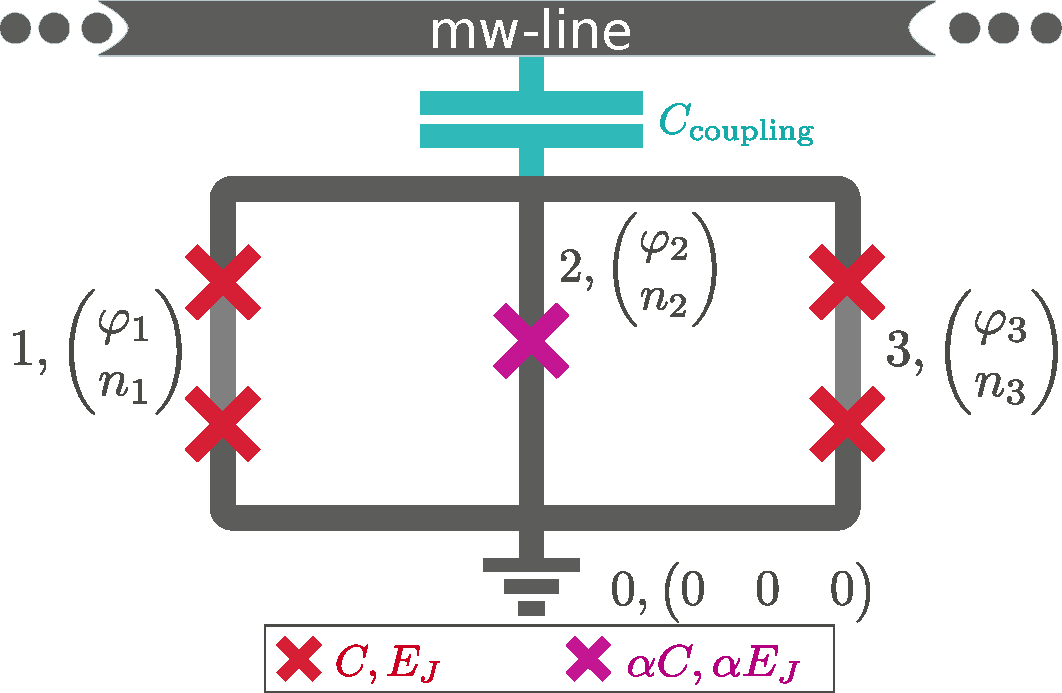
\includegraphics[width=100mm]{fig1_supp}
  \caption{\textbf{Topology of the twin flux qubit.}\label{fig:supp1}}
\end{figure}

The capacitance matrix couples charges on the islands $2e\vec{n} = 2e\{ n_1, n_2, n_3\}$ with their potentials $\vec{V} = \{ V_1, V_2, V_3\}$ according to $2e\vec{n} = \bold{C} \vec{V}$ and an electrostatic energy of the qubit is simplified to kinetic (phase dynamics) 
\begin{equation}
T= E_C C \vec{n}^T \bold{C}^{-1} \vec{n}, 
\end{equation}
where the charging energy $E_C = \frac{(2e)^2}{2C}$. The potential energy due to Josephson junction is 
\begin{equation}
U = E_J [4 + \alpha - \alpha \cos{\varphi_2} - \cos{\varphi_1} - \cos{\varphi_3} - \cos{(\varphi_2 - \varphi_1 - \varphi_{ext})} - \cos{(\varphi_2 - \varphi_3 + \eta \varphi_{ext})}].  
\end{equation}

\section{Representation of Hamiltonian in the charge basis}
\label{sec:repr-hamilt-charge}

We represent the system Hamiltonian $H=T+U$ in the charge basis.  
Taking into account the phase operator form $e^{\pm i\varphi} = \ket{n\pm 1}\bra{n}$ and omitting constants in the potential energy, the Hamiltonian is transformed to 
%\begin{eqnarray}
\begin{align}
H = E_C C \vec{n}^T &\bold{C}^{-1} \vec{n} -\frac{E_J}{2}\big(\alpha\ket{n_2+1}\bra{n_2}+\ket{n_1+1}\bra{n_1}+ \ket{n_3+1}\bra{n_3} + \nonumber\\
       & + e^{-i\varphi_{ext}}\ket{n_1-1,n_2+1}\bra{n_1,n_2} + e^{+i\eta\varphi_{ext}}\ket{n_2+1,n_3-1}\bra{n_2,n_3} + c.c. \big)
\end{align}
%\end{eqnarray}


%\begin{framed}\noindent
%  Here, we show how to represent the Hamiltonian of the system in matrix form for the charge basis, Fig~\ref{fig:matrix_representation}.
%\end{framed}
%
%\noindent The Hamiltonian
%
%\begin{equation}
%  \label{eq:hamitlian_revisited}
%  \begin{aligned}
%    \mathcal{H} & = T + U\\
%    & = E_C \iabs{C} \vec{n}^T\bold{C}^{-1}\vec{n} \\
%    & \quad+  E_J\big[4 + \alpha - \alpha\cos(\varphi_{2}) -\cos(\varphi_{1}) -\cos(\varphi_{3}) - \\
%    &  \qquad  \cos(\varphi_{2}   -  \varphi_{1}  -  \varphi_{\text{ext}})  -  \cos(\varphi_{2}   -  \varphi_{3}  +
%    \varphi_{\text{ext}})\big]
%  \end{aligned}
%\end{equation}

%\noindent in the charge basis  takes the  form  shown in  Fig.~\ref{fig:matrix_representation}, where a state \iket{-1, 0,  1} would correspond to a Cooper pair (CP) occupation of -1, 0 and 1 on islands 1, 2 and 3. Kinetic terms  ($ {T}(n_1, n_2, n_3  $) naturally  fall on  the diagonal  axis of  the matrix. The phase-dependent term ($ U(\varphi_1,\varphi_2,\varphi_3,\varphi_{\text{ext}})  $) are represented using the following procedure:
%
%\begin{enumerate}
%\item Derive  the commutation relation  between the number, $  \hat{n} $, and  the exponential
%  phase,     $    e^{\pm     i\hat{\varphi}}     $,    by     using     the    standard     relation
%  $ \left[\hat{n},\hat{\varphi}\right] = 1 $:
% 
%  {\scriptsize\begin{equation}\label{eq:ab1}
%      \begin{aligned}
%        \icommutation{\hat{\red{n}}}{e^{\pm i \hat{\blue{\varphi}}}} & =  \icommutation{\hat{n}}{\sum_{\alpha = 0}^{\infty} \frac{(\pm i\hat{\blue{\varphi}})^\alpha}{\alpha!}} = \sum_{\alpha = 0}^{\infty} (\pm i)^\alpha\frac{\icommutation{\hat{\red{n}}}{\hat{\blue{\varphi}}^\alpha}}{\alpha!}\\
%        &  = \sum_{\alpha  = 0}^{\infty}  (\pm i)^\alpha\frac{-\alpha  i\hat{\blue{\varphi}}^{\alpha -  1}}{\alpha!}  =  \pm \sum_{\alpha  =
%          1}^{\infty}i^{\alpha  -  1}\frac{(\pm\hat{\blue{\varphi}})^{\alpha  -  1}}{(\alpha   -  1)!}   =  \pm  e^{\pm
%          i\hat{\blue{\varphi}}}.
%      \end{aligned}
%    \end{equation}}
%
%\item Operating with the number operator on state $ e^{\pm i\hat{\blue{\varphi}}}\ket{n} $ and using
%  the commutation result \begin{equation}\label{eq:ab2}
%    \begin{aligned}
%      \hat{\red{n}}\bigg[e^{\pm   i\hat{\blue{\varphi}}}\ket{n}\bigg]    =   &    \bigg[\pm   e^{\pm
%        i\hat{\blue{\varphi}}}   +  e^{\pm   i\hat{\blue{\varphi}}}\hat{n}\bigg]\ket{n}  \\   &  =   (n\pm
%      1)\bigg[e^{\pm i\hat{\blue{\varphi}}}\ket{n}\bigg].
%    \end{aligned}
%  \end{equation}
%
%\item Evidently, the exponential phase operator is a ladder operator for the \iket{n} state:
%  \begin{equation}
%    \label{eq:ab5}
%    e^{\pm i\hat{\blue{\varphi}}}\ket{n} = \ket{n \pm 1} \Rightarrow e^{\pm i\blue{\varphi}} = \sum_{{n}} \iketbra{n\pm1}{n}.
%  \end{equation}
% 
%\item Thus  operator $\cos(\hat{\varphi}_2-\hat{\varphi}_1-\hat{\varphi}_{\text{ext}})$ can be  expressed in the
%  number basis $ \left\{n_{1},n_2,n_3\right\} $ as: {\scriptsize
%    \begin{equation}
%      \label{eq:ab4}
%      \begin{aligned}
%	\cos(\hat{\varphi}_2-& \hat{\varphi}_1-\hat{\varphi}_{\text{ext}}) =\\
%        & = \frac{1}{2}\left(e^{i\hat{\varphi}_{2}}e^{-i\hat{\varphi}_1}e^{-i\hat{\varphi}_{\text{ext}}}+\text{c.c.}\right)\\
%        & =  \frac{1}{2} \left(\left[\sum_{n_2}\iketbra{n_2+1}{n_2}\right]\right. \\
%        & \qquad \left.\otimes \left[\sum_{n_1}\iketbra{n_1-1}{n_1}\right]
%          \otimes\mathbb{I}^{(3)}\right)e^{-i\varphi_{\text{ext}}} + \text{c.c.}\\
%        &             =              \frac{1}{2}e^{-i\varphi_{\text{ext}}}             \sum_{n_{1,2,3}}
%        \iketbra{n_1-1,n_2+1,n_3}{n_1,n_2,n_3} + \text{c.c.}
%     \end{aligned}
%    \end{equation}}
  
%\item Physically this last term corresponds  to a CP exchange between island 1 and  island 2. An example
%  of a term could be
%  \begin{equation}
%    \label{eq:ab6}
%    \frac{1}{2}e^{-i\varphi_{\text{ext}}}\iketbra{-1,1,0}{0,0,0} + \frac{1}{2}e^{+i\varphi_{\text{ext}}}\iketbra{0,0,0}{-1,1,0},
%  \end{equation}
%  \noindent  which would  be a  pair of  symmetrical off-diagonal  elements in  the matrix  of
%  Fig.~\ref{fig:matrix_representation}.
%\end{enumerate}

Physically one before the last term corresponds  to a CP exchange between island 1 and  island 2. An example
  of a term could be
  \begin{equation}
    \label{eq:ab6}
    \frac{1}{2}e^{-i\varphi_{\text{ext}}}\iketbra{-1,1,0}{0,0,0} + \frac{1}{2}e^{+i\varphi_{\text{ext}}}\iketbra{0,0,0}{-1,1,0},
  \end{equation}
  \noindent  which would  be a  pair of  symmetrical off-diagonal  elements in  the matrix  of
  Fig.~\ref{fig:matrix_representation}.

\begin{figure}[h]
  \includegraphics[width=120mm]{fig4}
  \caption{\small \textbf{Hamiltonian in the CP-basis representation for 3-CP-states-per-island (27 system states):} Purple square denote the kinetic terms that all fall on the main diagonal. Light blue squares denote simple off-diagonal terms distributed symmetrically about the main diagonal, arising from e.g. $\cos(\varphi_2)$. Dark blue squares are have an additional flux dependence $e^{i\varphi_{\text{ext}}}, e^{i\eta\varphi_{\text{ext}}}$, arising from e.g. $\cos(\varphi_2-\varphi_1-\varphi_{\text{ext}})$.
    \label{fig:matrix_representation} }
\end{figure}


To decide on the number of states for the simulation, we took a sufficiently complete system state of 19 interacting CPs, and methodically ``switched off'' interactions between the high-CP-number states. Further increase, of the number of states does not improve accurate of calculations. We logged the deviation of the energy spectra of Fig.~\ref{fig:minimum_number}, where it shows that 9-CP-states describes the system almost as good as with the complete system state.

\begin{figure}[h]
  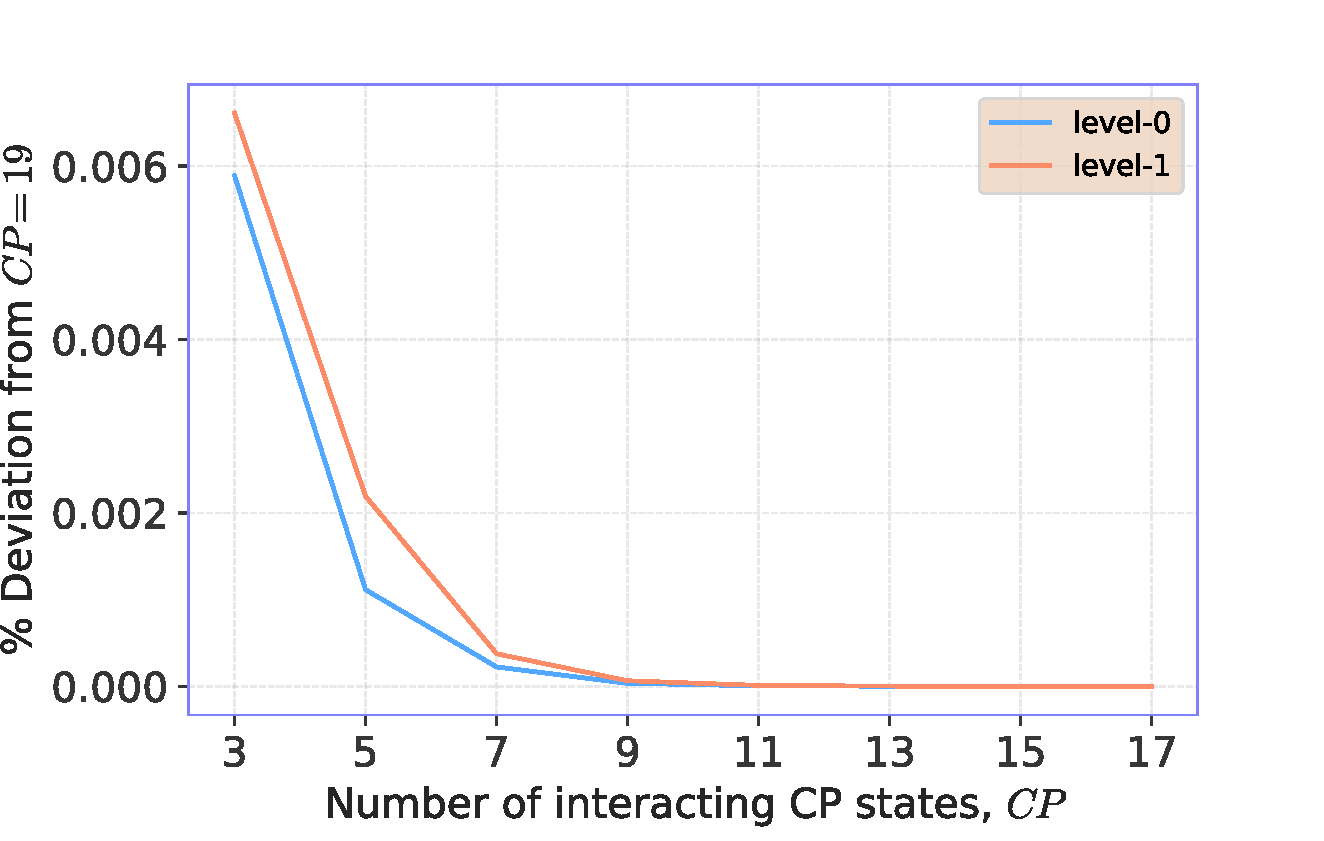
\includegraphics[width=86mm]{fig7}
  \caption{\small \textbf{Choosing the lowest number of interacting CP, that would  capture the nature of perturbation effects:} The energy levels for state \iket{0} (blue) and \iket{1} (red) were simulated for different numbers of interacting CP and compared to the simulation with 19CP (which we assume to be the most accurate and most intense simulation for the system). Consistency was reached for simulations with 9CP.
    \label{fig:minimum_number} }
\end{figure}

% For        example         $        \cos(\varphi_{2})         $        becomes
% $    \mathbb{I}_{1}\otimes\frac{1}{2}\left[\sum_{n_2}\iketbra{n_2+1}{n_2}    +
%   \iketbra{n_2-1}{n_2}   \right]\otimes\mathbb{I}_{3}    $,   where   identity
% operators $ \mathbb{I}_{1,3} $ carry the states of the non-involved islands.

\section{Transition matrix elements}
\label{sec:trans-matr-elem}

\begin{framed}\noindent
  Here we derive the transition matrix element used in the main paper
      \begin{equation}
    \label{eq:dipole_voltage_6}
    \ibra{g}\hat{V}_2 \iket{e} \equiv \frac{E_{C}}{2 e (1+\alpha)}\ibra{g}\left[\hat{n}_1  +  2\hat{n}_{2}
        +\hat{n}_3 \right]\iket{e}.
  \end{equation}
\end{framed}

Microwaves   in  the  transmission  line,   with  voltage
$   V_{\text{mw}}=   \iabs{V_{\text{mw}}}\cos(\omega_{21   }t)   $  are   coupled   via the coupling capacitor
$C_{\text{c}}$  to   the  qubit. Transitions \iket{1}~\ilra~\iket{2} stimulated by
this driving  generate a qubit voltage  of $  V_2 = \ibra{1}\hat{V}_2\iket{2} $ 

Expressing the voltage on the different islands:
  \begin{equation}
    \label{eq:dipole_voltage_8}
    \begin{aligned}
      \begin{pmatrix}
        V_{1}\\V_{2}\\V_{3}
      \end{pmatrix}  =  \vec{V}  =   \vec{Q}C^{-1}  &  =2eC^{-1}\vec{n}  =  \frac{2e}{\iabs{C}
      }\begin{pmatrix}
          2 & -1 & 0\\
          -1 & 2 + \alpha & -1\\
          0 & -1 & 2
        \end{pmatrix}^{-1} \begin{pmatrix} n_{1}\\n_{2}\\n_{3}
      \end{pmatrix}\\
      & = \frac{2e}{\iabs{C}} \frac{1}{4 + 4\alpha}\begin{pmatrix}
          3 + 2\alpha & 2 & 1\\
          2 & 4 & 2\\
          1 & 2 & 3+2\alpha
        \end{pmatrix} \begin{pmatrix} n_{1}\\n_{2}\\n_{3}
      \end{pmatrix}
          \end{aligned}
  \end{equation}

  \noindent one can read off

  \begin{equation}
        \begin{aligned}
      \hat{V}_2 &  = \frac{e}{C(1+\alpha)}  \left[ \hat{n}_1  + 2\hat{n}_{2}
        +\hat{n}_3 \right].
    \end{aligned}
  \end{equation}
  Thus, the transition matrix element

    \begin{equation}
    \label{eq:dipole_voltage_6}
    d_{i,j} = \ibra{i}\hat{V}_2 \iket{j} \equiv \frac{E_{C}}{2 e (1+\alpha)}\ibra{i}\left[\hat{n}_1  +  2\hat{n}_{2}
        +\hat{n}_3 \right]\iket{j}.
  \end{equation}




% \section{Rabi oscillation measurements}
% \label{sec:rabi-oscill-meas}

% \noindent Rabi  oscillations are observed when  a qubit system, with  a transition frequency
% $\omega_{21}$, is driven by microwaves in  resonance with this transition.  The expectation value
% of  $ \iaverage{\sigma_{-}}  $, $\sigma_{-}=\iketbra{0}{1}$,  which is  measured by  a vector  network
% analyzer \cite{Astafiev_2010}, oscillates sinusoidally with the  length of the drive as shown
% below.

% \begin{enumerate}
% \item The Hamiltonian during microwave driving of the system is a combination of the qubit's
%   two-level system Hamiltonian
%   \begin{equation}
%     \label{eq:rabi1}
%     \mathcal{H}_{q} = -\frac{\hbar\omega_{21}}{2}\sigma_{z},
%   \end{equation}

%   \noindent                                                                            where
%   $\sigma_z = \ensuremath{\left(\begin{smallmatrix} 1  & 0\\0 & -1 \end{smallmatrix}\right)}
%   $, and the Hamiltonian of the resonant drive of strength $ \hbar\Omega $
%   \begin{equation}
%     \label{eq:rabi2}
%     \mathcal{H}_{d} = \hbar\Omega\cos(\omega_{21}t)\sigma_{x}
%   \end{equation}

%   \noindent   that    couples   the   two    levels   through   the    transition   operator
%   $\sigma_x = \ensuremath{\left(\begin{smallmatrix} 0 & 1 \\ 1 & 0 \end{smallmatrix}\right)}
%   $.

% \item              Applying              the             unitary              transformation
%   $     U(t)    =     \exp    \left(-i     \frac{\omega_{21}t}{2}\sigma_z\right)    $     to
%   $ \mathcal{H} = \mathcal{H}_{q}+\mathcal{H}_{d} $ evaluates to
%   \begin{equation}
%     \label{eq:rabi3}
%     \begin{aligned}
%       \mathcal{H}'& = U\mathcal{H}U^{\dag} - i\hbar U\dot{U}^{\dag}\\
%       & \approx \frac{\hbar\Omega}{2}\sigma_x
%     \end{aligned}
%   \end{equation}

%   \noindent    under     the    approximation     that    non-conserving     energy    terms
%   $ e^{\pm 2i\omega_{21}t} $ are neglected.
  
% \item  The evolution  of  a  ground state  in  this  rotated frame  for  a  drive of  length
%   $ \Delta t $ is
%   \begin{equation}
%     \label{eq:rabi4}
%     \begin{aligned}
%       U'(\Delta t)\iket{0} & = e^{-i\frac{\mathcal{H'}}{\hbar}\Delta t}\iket{0} \\
%       &     =      \cos\left({\Omega\Delta     t}/{2}\right)\ket{0}+i\sin\left({\Omega\Delta
%         t}/{2}\right)\ket{1},
%     \end{aligned}
%   \end{equation}

%   \noindent which as a density matrix reads

%   \begin{equation}
%     \label{eq:rabi6}
%     \rho_{\Delta t} = \frac{1}{2}\begin{pmatrix}
%       1 + \cos(\Omega\Delta t) & -i\sin(\Omega\Delta t)\\
%       i\sin(\Omega\Delta t) & 1 - \cos(\Omega\Delta t)
%     \end{pmatrix}
%   \end{equation}

%   \noindent

% \item Rabi oscillations, proportional, to $ \iaverage{\sigma_{-}} $:
%   \begin{equation}
%     \label{eq:rabi5}
%     \begin{aligned}
%       \iaverage{\sigma_{-}} & = \bra{0}U'^{\dag}(t) \iketbra{0}{1} U'(t)\iket{0}\\
%       & = \sin \left(\Omega t\right)
%     \end{aligned}
%   \end{equation}

% \end{enumerate}

\end{document}
